\chapter{Bistability  and  Hysterisis in Dynamical Systems: COMING SOON}
\label{ch-bistability}

Bistability and hysteresis many physical phenomena. Below, we'll give examples of dynamical systems (i.e., systems of ordinary differential equations, SODE) with 2 or 3 dofs 
(degrees of freedom) with these properties.

\begin{figure}[h!]
\centering
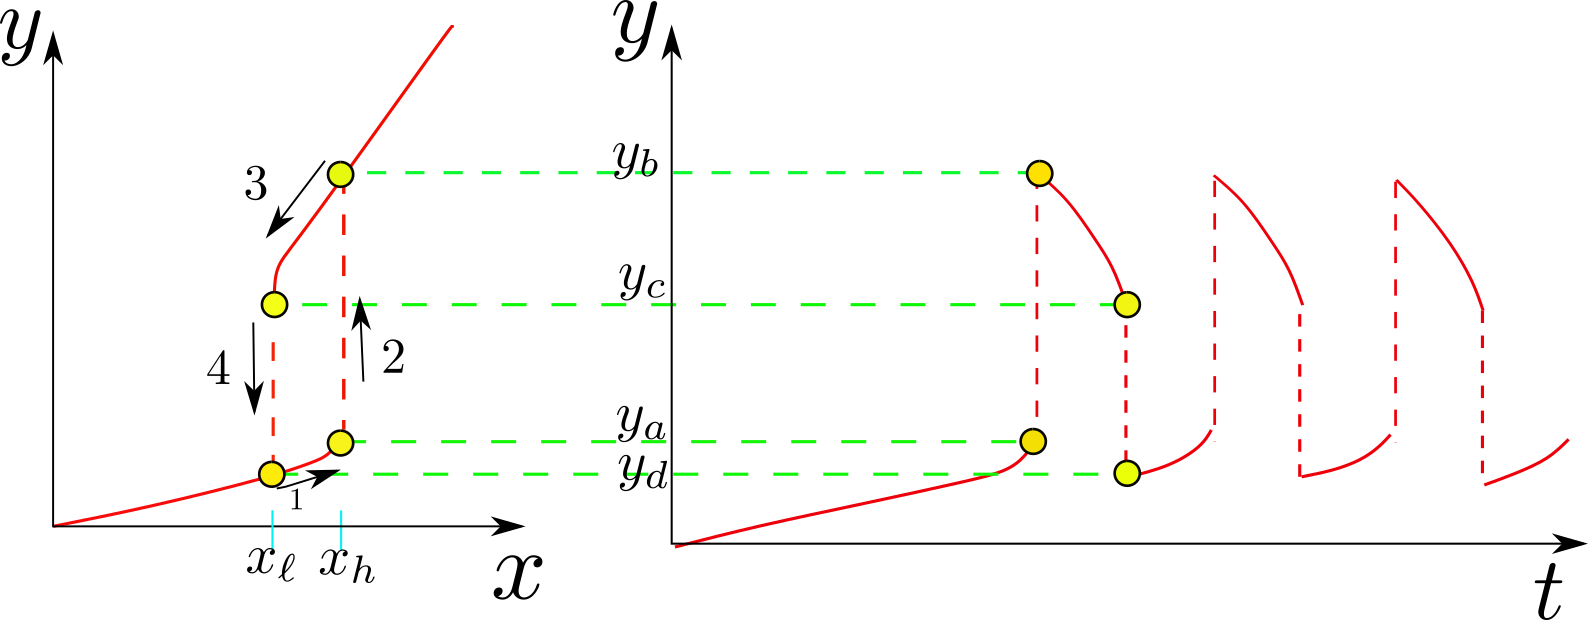
\includegraphics[width=5in]
{bistability/hysterisis.png}
\caption{Hysterisis. $x$ represents an input and $y$ an output. $t$ represents time.}
\label{fig-hysterisis}
\end{figure}

\section{Lorenz System }

The  {\bf Lorenz system} arises in fluid mechanics and laser physics, and other places.
It is given by


\begin{figure}[h!]
$$
\xymatrix@R=3pc@C=3pc{
\rvy\ar[d]|\redminus
\ar[r]
\ar@[green]@/^.8pc/[drr]|\redplus
&\bigotimes\ar[drrr]|\redplus
&\rvx\ar[l]
\ar[r]
\ar[d]|\redminus
\ar@[green]@/_.8pc/[dll]|\redplus
&\bigotimes\ar[dlll]|\redminus
&\rvz\ar[d]|\redminus
\ar[l]
\\
\dot{\rvy}
&&\dot{\rvx}
&&\dot{\rvz}
}$$
\caption{Lorentz system. \OTO}
\label{fig-lorenz-sys}
\end{figure}

\beq
\left\{
\begin{array}{l}
\dot{x} = \sigma (y - x)
\\
\dot{y} = x(\rho - z) - y
\\ 
\dot{z} = xy - \beta z
\end{array}
\right.
\eeq

where $\sigma > 0$, $\rho > 0$, and $\beta > 0$ are parameters.

For certain parameter values (e.g., $\sigma = 10, \beta = 8/3, \rho \in [24, 30]$), the Lorenz system exhibits bistability and hysteresis. In this regime, the system has two coexisting attractors (such as chaotic attractors or fixed points) and can jump between them depending on initial conditions and parameter sweeps. This transition can exhibit hysteresis as $\rho$ is increased or decreased.



\section{FitzHugh-Nagumo model}
The {\bf FitzHugh-Nagumo model} is a reduced form of the Hodgkin-Huxley model for neuronal dynamics. It is given by

\begin{figure}[h!]
$$
\xymatrix@R=3pc@C=3pc{
\rvx^3\ar[dr]|\redminus
&\rvx\ar[d]|{\;\redplus}
 \ar[dr]|\redplus
 \ar[l]
& \rvy\ar[d]|\redminus
\ar@/_1pc/[dl]|\redminus
\\
\ar[r]|\redplus
&\dot{\rvx}
&\dot{\rvy}
&\ar[l]|\redplus
}
$$
\caption{FitzHugh-Naguno model. \OTO}
\label{fig-fitz}
\end{figure}

\beq
\left\{
\begin{array}{l}
\dot{x} = x - \frac{x^3}{3} - y + R
\\
\dot{y} = \frac{1}{\tau} (x + a -b y)
\end{array}
\right.
\eeq



\section{Genetic Toggle Switch}
A  {\bf genetic toggle switch}
can be described by:

\begin{figure}[h!]
$$
\xymatrix@C=3pc@R=4pc{
\rvx\ar[dr]|\redoplus
\ar[d]|\redminus
&\rvy\ar@/_1pc/[dl]|\redoplus
\ar[d]|\redminus
\\
\dot{\rvx}
&\dot{\rvy}
}$$
\caption{Genetic Toggle Switch. \OTO}
\label{fig-gene-toggle}
\end{figure}

\beq
\left\{
\begin{array}{l}
\dot{x} = \frac{\alpha_1}{1 + \left(\frac{y}{K_1}\right)^{n_1}} - \gamma_1 x
\\
 \dot{y} = \frac{\alpha_2}{1 + \left(\frac{x}{K_2}\right)^{n_2}} - \gamma_2 y
\end{array}
\right.
\eeq

where $x$, $y$, and $z$ represent concentrations of proteins, $\alpha_1, \alpha_2, \alpha_3 > 0$ are production rates, and $n, m, p > 1$ control the steepness of the repression.
